%------------------------------------------------------------------------------
% Template file for the submission of papers to IUCr journals in LaTeX2e
% using the iucr document class
% Copyright 1999-2013 International Union of Crystallography
% Version 1.6 (28 March 2013)
%------------------------------------------------------------------------------

\documentclass[]{iucr}              % DO NOT DELETE THIS LINE
     %-------------------------------------------------------------------------
     % Information about journal to which submitted
     %-------------------------------------------------------------------------
     \journalcode{J}              % Indicate the journal to which submitted
                                  %   A - Acta Crystallographica Section A
                                  %   B - Acta Crystallographica Section B
                                  %   C - Acta Crystallographica Section C
                                  %   D - Acta Crystallographica Section D
                                  %   E - Acta Crystallographica Section E
                                  %   F - Acta Crystallographica Section F
                                  %   J - Journal of Applied Crystallography
                                  %   M - IUCrJ
                                  %   S - Journal of Synchrotron Radiation

\usepackage{verbatim}
\usepackage{graphicx}
\usepackage{tikz}
\usepackage{amsmath}
\usepackage{amsfonts}
\usepackage{listings}
\usepackage{color,soul}

\lstset {
	frame=single
}
\lstdefinelanguage{ini} {
	basicstyle=\ttfamily\scriptsize,
	columns=fullflexible,
	morecomment=[s][\color{red}\bfseries]{[}{]},
	morecomment=[l]{\#},
	commentstyle=\color{blue}\ttfamily,
	morekeywords={},
	otherkeywords={=,:::},
	keywordstyle={\color{blue}\bfseries}
}

\begin{document}                  % DO NOT DELETE THIS LINE
     %-------------------------------------------------------------------------
     % The introductory (header) part of the paper
     %-------------------------------------------------------------------------

     % The title of the paper. Use \shorttitle to indicate an abbreviated title
     % for use in running heads (you will need to uncomment it).

\title{The Expand-Maximize-Compress Single Particle Imaging Algorithm}
%\shorttitle{Short Title}

     % Authors' names and addresses. Use \cauthor for the main (contact) author.
     % Use \author for all other authors. Use \aff for authors' affiliations.
     % Use lower-case letters in square brackets to link authors to their
     % affiliations; if there is only one affiliation address, remove the [a].

\author[a]{Kartik}{Ayyer}

\author[b]{Ti-Yen}{Lan}

\author[b]{Veit}{Elser}

\cauthor[c]{N. Duane}{Loh}{duaneloh@nus.edu.sg}

\aff[a]{Center for Free-Electron Laser Science, Deutsches Elektronen-Synchrotron DESY, Notkestra{\ss}e 85, 22607 Hamburg, \country{Germany}}
\aff[b]{Laboratory of Atomic and Solid State Physics, Cornell University, Ithaca, NY 14853 \country{USA}}
\aff[c]{Centre for Bio-imaging Sciences, National University of Singapore, 117543, \country{Singapore}}

     % Use \shortauthor to indicate an abbreviated author list for use in
     % running heads (you will need to uncomment it).

%\shortauthor{Soape, Author and Doe}

     % Use \vita if required to give biographical details (for authors of
     % invited review papers only). Uncomment it.

%\vita{Author's biography}

     % Keywords (required for Journal of Synchrotron Radiation only)
     % Use the \keyword macro for each word or phrase, e.g. 
     % \keyword{X-ray diffraction}\keyword{muscle}

%\keyword{keyword}

     % PDB and NDB reference codes for structures referenced in the article and
     % deposited with the Protein Data Bank and Nucleic Acids Database (Acta
     % Crystallographica Section D). Repeat for each separate structure e.g
     % \PDBref[dethiobiotin synthetase]{1byi} \NDBref[d(G$_4$CGC$_4$)]{ad0002}

%\PDBref[optional name]{refcode}
%\NDBref[optional name]{refcode}

\maketitle                        % DO NOT DELETE THIS LINE

\begin{synopsis}
Description of a single-particle X-ray imaging reconstruction and simulation package named EMC.
\end{synopsis}

\begin{abstract}
Single Particle Imaging (SPI) with X-ray Free-Electron Lasers (XFEL) can fundamentally change how we image bio-macromolecules. If SPI were to become routine, we can collect millions of diffraction patterns from single macromolecules before radiation damage rends each of them apart. The complexity of this resultant data stream is staggering: these millions of incomplete, noisy and un-oriented patterns must be computationally assembled for us to reconstruct the macromolecule's three-dimensional structure {\it de novo}. In this paper, we describe a software package based on a parallel implementation of the Expand-Maximize-Compress reconstruction algorithm that can complete this computational assembly for SPI. An auxiliary package to simulate SPI data streams is also included in this package, using which we demonstrate the feasibility of SPI at the Linac Coherent Light Source. We conclude by discussing diagnostics for determining the convergence of such SPI reconstructions, and future work planned for this package.
\end{abstract}


     %-------------------------------------------------------------------------
     % The main body of the paper
     %-------------------------------------------------------------------------
     % Now enter the text of the document in multiple \section's, \subsection's
     % and \subsubsection's as required.

\section{Introduction}

Experiments performed in 2015 at Linac Coherent Light Source (LCLS) \cite{Aquila2015} have demonstrated that single particle imaging (SPI) of large biomolecules at resolutions approaching $5 \,\AA$ is nearly at hand\footnote{Manuscript in preparation.}. To prepare for a future where SPI is routine, we are making available a software package that will make this new imaging modality accessible to a broad user base.

By now the defining characteristics of an SPI experiment are well known \cite{Neutze2000}: collect individual noisy diffraction patterns from very many reasonably identical copies of a particle, injected with unknown orientations into a pulsed x-ray beam. The Expand-Maximize-Compress (EMC) algorithm \cite{loh2009} was developed specifically for processing SPI data sets. It was designed to take advantage of all the available information in these experiments while also scaling well computationally. To get a better sense of the information processing advantages of EMC, we briefly contrast it with two alternative methods that have been proposed.

Manifold embedding methods \cite{Schwander2012} try to find a consistent set of particle orientations by identifying similar pairs of diffraction patterns that establish an adjacency network for embedding into the space of orientations. Nowhere does this method impose consistency between the many more pairs of diffraction patterns that are not similar. By contrast, EMC imposes consistency between each diffraction pattern and a 3D intensity model built from a tentative orientation reconstruction of \textit{all} the patterns.

Intensity cross-correlation methods offer another approach for deriving structure from un-oriented particle ensembles \cite{Kam1977, Saldin2010}. These methods work best when the x-ray flux passes through the fewest number of particles. However, in the single particle limit these methods work at an enormous information deficit relative to EMC. That is because EMC uses the correlated arrangement of \textit{all} 100-1000 photons in a typical diffraction pattern rather than just the correlations among pairs.

While EMC is just beginning to be used for SPI of bio-particles, it has been field-tested in a number of proof-of-principle experiments \cite{philipp2012,ayyer2014,wierman2016}. The most significant feature of these experiments is the demonstration that EMC's probabilistic modeling of the detector photon counts continues to be valid even in the extremely sparse regime. Recording highly sparse data, with the hope that it reveals structure, will require a leap of faith on the part of structural biologists. Our EMC software package comes with tools to make that leap less blind for new users.

     %-------------------------------------------------------------------------
     % Purpose and structure of this package
     %-------------------------------------------------------------------------

\section{Purpose and structure of this package}\label{sec:package}

This software package uses the EMC algorithm to reconstruct a 3D diffraction volume from noisy, randomly-oriented single particle diffraction (SPI) patterns. These patterns could be from simulations or actual single-particle experiments. Although this package includes a data stream generator that feeds data into the EMC reconstruction algorithm, the algorithm can also take data from physical experiments as long as the input/output formats specified here are used.

\subsection{Key parameters in single particle imaging}\label{sec:expParams}

The key parameters of an SPI experiment are illustrated in Figure \ref{fig:expGeometry}, which include the photon wavelength $\lambda$ and the maximum scattering angle $\phi_{\text{max}}$. These parameters determine the half period resolution $a$ of the reconstructed electron density map. Given these parameters together with the beam fluence, one can then decide if a candidate scatterer can yield enough diffraction signal to the desired resolution. These parameters are revisited in Section \ref{subsubsec:config}.

Throughout this document, we adopt the crystallographers' convention for the spatial frequency 
\begin{equation}
\widehat{q} = \frac{2 \sin(\phi_{\text{max}}\,/\,2)}{\lambda}\;.
\end{equation}
A corrective factor is applied to compensate for different solid angles subtended by different pixels on the detector (Appendix \ref{sec:solidAngle}). 

\subsection{Reconstruction workflows}\label{sec:dataStreamSim}

Whether the diffraction patterns are derived from simulations (Figure \ref{fig:simFlowchart}) or experiments (Figure \ref{fig:expFlowchart}), the minimum input to this reconstruction package are: a configuration file, a file containing detector coordinates plus pixel status, and a sparse representation of the photon data from diffraction patterns. 

Modules in this package can be replaced by alternatives with compatible input and output data formats with other modules. In this package, binary files have extensions \texttt{*.bin} or \texttt{*.emc}; plain text files terminate with \texttt{*.log}, \texttt{*.dat}, or \texttt{*.ini}.

\subsection{Implementing the EMC algorithm}\label{subsec:EMC}
The EMC algorithm \cite{loh2009} is implemented here with hybrid MPI+OpenMP, and hence suitable for both shared and distributed memory systems. In this section, we describe this implementation and an extension to deal with high signal data. 

In the current version, the code assumes a Poisson probability model for the number of photons in a pixel. 
%This means that if the mean number of photons at a pixel is $W$, the probability of getting $K$ photons is given by
%\begin{equation}
%P(K{\big\vert}W) = \frac{W^K e^{-W}}{K!}\;.
%\end{equation}
Gaussian noise models have been used in situations with bright, but noisy data \cite{loh2010,ekeberg2015}, but if single photons can be accurately counted, the noise model will be Poissonian. 

We consider the Poisson noise model for a set of 3D intensities $W$. Let the number of photons at pixel number $t$ in 2D data frame (interchangeably termed {\it photon/diffraction pattern}) $d$ be $K_{dt}$, and for a given orientation $r$ the predicted mean intensity at the same pixel be $W_{rt}$. Since an independent Poisson process occurs at each pixel, the probability of that pattern being generated by tomogram $W_r$ is
\begin{equation}
R_{dr} = \prod_t \frac{W_{rt}^{K_{dt}} e^{-W_{rt}}}{K_{dt}!} \;.
\label{eqn:probnumr}
\end{equation}
But since the particle must have some orientation, the probability of frame $d$ having orientation $r$ is obtained by normalizing over all orientations:
\begin{equation}
P_{dr} = \frac{R_{dr}}{\sum\limits_r R_{dr}}\;.
\label{eqn:prob}
\end{equation}
With these probabilities, one can define the model log-likelihood as the expectation of the total log-likelihood of the data being generated by a new model $W'_{rt}$
\begin{equation}
Q(W', W) = \sum_d \sum_r \sum_t P_{dr} (K_{dt} \log(W'_{rt}) - W'_{rt}) \;, 
\label{eqn:totalq}
\end{equation}
neglecting a model-independent constant. Maximizing $Q$ with respect to the new model intensities $W'_{rt}$ gives us the update rule
\begin{equation}
W_{rt} \longrightarrow W'_{rt} = \frac{\sum\limits_d P_{dr} K_{dt}}{\sum\limits_d P_{dr}}\;.
\label{eqn:wupdate}
\end{equation}

The most time-consuming step of each iteration is the calculation of Eq.~\ref{eqn:probnumr}. This involves comparing all the tomograms with all the patterns for each pixel which has at least one photon. The code is parallelized over orientations, so each MPI and OpenMP rank performs the calculation for a subset of orientations. At the start of the iterations, each MPI rank gets a copy of the current 3D intensity model $W$. Each MPI and OpenMP rank then calculates the relevant tomograms, $W_{rt}$, as needed and then computes $R_{dr}$ for that orientation using Eq.~\ref{eqn:probnumr}. Subsequently, these $R_{dr}$ are synchronously reduced across all ranks for the normalization operation Eq.~\ref{eqn:prob}. The $P_{dr}$ array is then used to calculate updated tomograms for each $r$, and then merged to obtain an updated 3D model for each MPI rank. These models are then reduced to obtain an updated model $W'$.

In many experimental situations, the incident fluence varies between x-ray pulses. Thus, the tomograms would be scaled differently for each pattern \cite{loh2010,ekeberg2015}. One can enable the recovery of these scale factors using the update rule described in Appendix~\ref{sec:rescaling}. 

We also find that if the signal is too strong, and when rotation group sampling is too fine or data is too few, reconstructions get stuck in local maxima in which all frames are assigned the same orientation and overlap with each other in reciprocal space. This effect is similar to what is observed if the background is too high~\cite{ayyer2015}. Such reconstructions, however, are empirically stable around the true solution, $W^{\text{true}}$, and only falters when one starts from a random initial guess. This problem can be avoided by using the deterministic annealing variant of expectation maximization ~\cite{ueda1998}. In the EMC case, this is implemented by raising $R_{dr}$ calculated in Eq.~\ref{eqn:probnumr} to a small power $\beta$, and then normalizing similar to Eq.~\ref{eqn:prob}. This has a regularizing effect of broadening the orientation distribution and results in a rotationally blurred, but stable reconstruction. Once a metastable model intensities is resolved, the power $\beta$ can then be raised gradually in a manner similar to simulated annealing to slowly guide the reconstruction to the true global maxima around $W^{\text{true}}$. An example of this is shown in Section~\ref{subsec:regularization}.

\subsection{Modules and convenience utilities}\label{subsec:mod+utils}

The modules and utilities here are either written in C or Python (files with $*.py$ extensions). For system requirements to run the code, see Section~\ref{sec:access}.

\subsubsection{Modules}\label{subsubsec:mods}
Here are the essential modules for simulating a data stream from a single-particle imaging experiment. By default, these modules use parameters listed in a single \texttt{config.ini} configuration file, although different modules can use different configuration files as well.

\begin{enumerate}
\item{\bf make\_detector.py.} Creates a detector file using the experimental parameters specified in the configuration file. The format of this file is specified in Section~\ref{subsubsec:detector}.
\item{\bf make\_densities.py.} Creates an electron density map from an atomic model in the Protein Data Bank (PDB) format, given the resolution and field of view calculated from the configuration file. A low-pass filter is applied to this electron density map to effect the intensity fall-off of atomic form factors.
\item{\bf make\_intensities.py}. Creates a set of 3D diffraction intensities from an electron density map and the experimental parameters found in the configuration file.  
\item{\bf make\_data}. Simulates a sparse photon diffraction pattern using a 3D diffraction volume (e.g. the one generated by {\bf make\_intensities.py}), and the configuration file. By default these photon data are saved as a binary file, \texttt{photons.emc}, detailed in Section~\ref{subsubsec:emcformat}. One can include a pattern-wise Gaussian spread in the incident fluence on the particle as well as uniform background.
\item{\bf make\_quaternion}. Creates a list of quasi-uniform rotation group samples based on a refinement scheme of the 600-cell, as described in \citeasnoun{loh2009}. These samples are used by the {\bf emc} reconstruction algorithm, as instructed by the \texttt{config.ini} configuration file.
\end{enumerate}

\subsubsection{Convenience utilities}\label{subsubsec:utils}
Several convenience utilities are included to help prepare the data for or view the results from the EMC reconstruction algorithm. The function of these utilities, which are non-essential for the reconstruction be easily substituted, are briefly described here. 
\begin{enumerate}
\item{\bf init\_new\_recon.py.} This Python utility compiles the C executables in the package, and makes them and the rest of the utilities available in a newly initialized reconstruction sub-directory. Alternatively, a Makefile is also included for users who would like to customize this compilation.
\item{\bf sim\_setup.py.} This Python utility simulates an SPI data stream using the parameters listed in the configuration file. This utility, in turn, calls the following modules listed above: {\bf make\_densities.py}, {\bf make\_intensities.py}, {\bf make\_data.py}, and {\bf make\_quaternions}.
\item{\bf make\_powder.py}. Makes a virtual powder pattern from a large stack of diffraction patterns stored in the sparse photon format adopted in this package.
\item{\bf run\_emc.py}. Starts the EMC reconstruction by calling its MPI+OpenMP implementation in C. Includes a few convenience operations like calling the {\bf make\_quaternion} module to increase the sampling of the rotation group and registering this increase in the configuration file before starting a reconstruction.
\item{\bf autoplot.py}. Renders the results of the EMC reconstruction, including the diagnostics it generates, with the option of automatically updating the plots when newer intensities become available.
\end{enumerate}


\subsection{Configuration and data formats}\label{subsec:formats}

We outline only the data formats for the input and output in Figure \ref{fig:expFlowchart}. The formats for the data stream generator, which are auxiliary to the reconstruction algorithm, are detailed in the distributed software package. 

\subsubsection{Configuration file}\label{subsubsec:config}

The plain-text configuration file contains parameters and file names to be used by the EMC reconstruction as well as the various modules/utilities. The file has the standard \texttt{key = value} format with the parameters for different modules grouped by module names in square brackets. There is a global \texttt{[parameters]} section containing information about the experimental setup. A typical configuration file is shown in Fig.~\ref{fig:config}, which corresponds to the first simulation case in Table \ref{table:simParams}. This default file also shows the use of special keywords used to point to other configuration file parameters (eg. \texttt{in\_photons\_file}). The \texttt{[parameters]} section is described below. For other sections, refer to the appropriate module in Section~\ref{subsec:mod+utils}.

The basic parameters of the experiment are:
\begin{itemize}
\item \texttt{detd}: Detector distance in mm.
\item \texttt{lambda}: Wavelength in \AA.
\item \texttt{detsize}: Detector size (assuming square detector) in pixels.
\item \texttt{pixsize}: Pixel size in mm.
\item \texttt{stoprad}: Radius of beamstop in pixels.
\item \texttt{polarization}: Polarization direction of the x-ray pulses (can be x, y, or none).
\end{itemize}



\subsubsection{Detector file}\label{subsubsec:detector}
The detector file is an ASCII (human readable) file which describes various properties of the detector. The first line of the file specifies the number of pixels. Subsequently, individual pixels are described by five columns of numbers, one pixel per line. The first three columns give the 3D coordinates of the detector pixel in voxels, where the voxels refer to the 3D grid containing the intensity model. The fourth column gives the product of the polarization and solid angle corrections for that pixel (Appendix \ref{sec:solidAngle}). The last column is an 8-byte unsigned integer whose value is used by the EMC code as well as other utilities to categorize the pixel. Currently, there are three categories:
\begin{description}
\item[0]{Good pixels, used to determine the orientation of a given pattern and updated into the new intensity model.}
\item[1]{These pixels will not be used to determine the orientation, but will still be merged into the 3D grid using the orientations calculated from category 0 pixels. These are usually pixels in the corners of the detector.}
\item[2]{Bad pixel, which are either dead pixels or pixels within the beamstop. Their values will be used neither to determine the orientation nor to calculate the merged 3D intensities.}
\end{description}

\subsubsection{Photon file (emc format)}\label{subsubsec:emcformat}
Since the photon data in many high-resolution SPI experiments expect few photons per pattern, a sparse binary format is used to store the data. Hence, for each pattern we only store information of pixels that receive photons. Additionally, since most of the non-zero counts are ones, only their pixel locations are stored. For pixels receiving two or more photons, we store both their pixel location and photon count. 

Figure \ref{fig:dataFormat} shows a cartoon of this data format. These are arranged in six blocks. The file's header resides in the first block, which is 1024 bytes long. The first 4 bytes are a 32-bit integer giving the number of patterns (\texttt{num\_data}) contained in the file. The next 4 bytes are also a 32-bit integer giving the number of pixels in the detector file used to number the pixels. The next 1016 bytes are currently empty (filled with zeros).

The second block contains \texttt{num\_data} 32-bit integers giving the number of one-photon events in each pattern (\texttt{ones}). The third block contains \texttt{num\_data} integers giving the number of multi-photon events (\texttt{multi}). The total number of single photon events in all the patterns is the sum of all numbers in the \texttt{ones} array ($S_o$). Similarly, let $S_m$ be the total number of multiple photon events. The fourth block contains $S_o$ 32-bit integers giving the locations of the single photon pixels; the fifth block has $S_m$ integers with the locations of the multiple photon pixels. Finally, the sixth block has $S_m$ 32-bit integers giving the number of photons in each of those multiple photon pixels. 


     %-------------------------------------------------------------------------
     % Example reconstructions
     %-------------------------------------------------------------------------
     
\section{Example reconstructions of simulated experiments}\label{sec:simulations}

The use of our package is exemplified in three simulated single-particle imaging (SPI) reconstructions using the specifications of Atomic Molecular and Optical Science (AMO)~\cite{ferguson2015} and Coherent X-ray Imaging (CXI) ~\cite{liang2015} endstations at Linac Coherent Light Source (LCLS) \cite{Emma2010}. We chose to simulate SPI of keyhole limpet hemocyanin (KLH1) didecamer~\cite{gatsogiannis2009} and four-layer Tobacco Mosaic Virus (TMV)~\cite{bhyravbhatla1998} at AMO and CXI respectively. Notably, the choices in Table \ref{table:simParams} yield an average of $\sim 100$ photons per single-particle diffraction pattern.



The simulation parameters are shown in Table \ref{parameters}. The detectors here have $1024\times1024$ pixels, taking on the pixel pitch of the pnCCD\cite{Struder2010} and CSPAD\cite{hart2012} detectors. We decrease the beam fluence to obtain mean photon counts $N\sim 90$ for the first two simulations, mimicking realistic losses from imperfect beam transmission, optics, and cleanup apertures \cite{Loh2013}. The third simulation of Table \ref{table:simParams} was designed to demonstrate how deterministic annealing method can deal with convergence issues caused by very high signal. Most of the parameters were identical to the low fluence AMO simulation except the fluence was up-adjusted to receive 1 mJ x-ray pulses, which is within an order of magnitude of design specifications \cite{Emma2010}.

For data sufficiency we use the signal-to-noise ratio parameter defined in Eq. 37 of \citeasnoun{loh2009}, 
\begin{equation}
S = \sqrt{\frac{N M_{\text{data}}}{M_{\text{rot}}}}\; ,
\end{equation}
to estimate the required number of data frames $M_{\text{data}}$ for $S\sim50$, where $M_{\text{rot}}$ is the number of quasi-uniform rotation samples. Assuming the diffraction patterns are uniformly distributed in orientation space, $S^2$ can be interpreted as the average number of photons per orientation.

\subsection{Diagnostics on simulated reconstructions} \label{subsec:recon}
In this section, we describe useful diagnostics for monitoring the progress of each 3D reconstruction. Figures \ref{fig:amo_low_intens}, \ref{fig:cxi_intens} and \ref{fig:amo_high_intens} show orthogonal slices through the reconstructed intensities for the three parameter sets in Table \ref{table:simParams}. Below each figure is a set of plots generated by \texttt{autoplot.py} utility, which helps visualize these diagnostics. 

We discuss these diagnostics starting with the AMO reconstruction in Figure \ref{fig:amo_low_log}, which consistently converges from random restarts. With each new reconstruction attempt, diffraction speckles readily converge, although each time at a different overall orientation.

\subsubsection{R.M.S. change in the 3D model}
The root mean squared change per voxel between the 3D intensity models from successive iterations in Figure \ref{fig:amo_low_log} is a straightforward indicator of convergence. The model changes by smaller and smaller amounts as the algorithm converges on a solution.

\subsubsection{Mutual information between model and data}
An additional diagnostic is the sharpness of the probability distribution over orientations $P_{dr}$ calculated in Eq.~\ref{eqn:prob}. This can be assessed by calculating the mutual information of the joint distribution of the data and the orientations, $P(K,\Omega) = P(\Omega) P(K{\big\vert}\Omega) = P_r P_{dr}$. Here, $P_r$ is the prior probability of orientations (assumed here to be uniform). This quantity is evaluated as
\begin{equation}
I(K, \Omega) = \langle\sum_r P_{dr} \log(P_{dr} / P_{r})\rangle, \label{eq:mutualInfo}
\end{equation}
where $\langle \dots \rangle$ is the average over data frames. The quantity in Eq.~\ref{eq:mutualInfo} approaches the entropy of the rotation group sampling when each pattern fits only one orientation, while it vanishes for a uniform distribution. The fact that this quantity rises asymptotically in Figure ~\ref{fig:amo_low_log} (bottom panel, top plot) is consistent with model convergence. Below that is a plot of the model log-likelihood defined in Eq.~\ref{eqn:totalq}. In most situations, this quantity increases monotonically, and a significant decrease over many iterations indicates an error. 

\subsubsection{Most likely orientations of each pattern}
The bottom rightmost plot in Figure \ref{fig:amo_low_log} is the most useful for monitoring convergence. This is a matrix plot where the vertical axis is the frame number while the horizontal is iteration. The color represents the orientation number of the best orientation (maximum $P_{dr}$) for each frame. Thus, the colors at the right end form a smooth spectrum and the pattern numbers differ between rotation-sampling blocks. The variation of colors along a row indicates how the most likely orientation has changed for that frame. Patterns settle into their most likely orientations when these colors become constant with iterations, which is a good indicator of convergence.

This is also useful for cases when the rotation group sampling is steadily increased (i.e. Figure \ref{fig:cxi_intens}). For each iteration block where the rotation group sampling is fixed, we sort the patterns (rows in this orientation plot) such that the last iteration in the block has ascending orientation numbers. However, note that while the pattern index is constant within each block, they differ between blocks because each block is separately sorted.

\subsection{Strategies for reconstruction} \label{subsec:strategy}

\subsubsection{Gradually increasing rotation group sampling} \label{subsec:quatRefine}
For the CXI reconstruction (Fig.~\ref{fig:cxi_log}), due to the size of the problem, the quaternion sampling number was increased in steps. If one chooses too coarse a rotation group sampling, low resolution speckles get reconstructed but higher resolution features remain blurry. These higher resolution speckles quickly sharpen when we increase the rotation group sampling for reconstructions starting from this blurry model. Since the computation time scales as the number of rotation group samples, it is faster to slowly increase rotation group sampling such that only a few iterations are performed with the most time-consuming but finest sampling. Red dashed lines in the bottom plots of Fig.~\ref{fig:cxi_log} indicate iterations where the sampling rate was increased, starting from 10 and ending at 16. Note that the mutual information does not increase much in the last rotation group refinement, indicating that further refinement would not substantially improve model likelihood.

\subsubsection{Regularization via deterministic annealing} \label{subsec:regularization}
For the high fluence AMO reconstruction (Fig.~\ref{fig:amo_high_log}), the situation is slightly different. As mentioned before, due to very high signal, the algorithm can fall into a local maxima trap in the first few iterations. This can be avoided by starting with a low $\beta$ as described in Section~\ref{subsec:EMC}. This reduces the propensity for over-fitting at the start of the reconstruction. In this particular case $\beta$ was 0.001 for the first 10 iterations and was then doubled every 10 iterations. The black dashed lines represent the iterations at which $\beta$ was doubled. After 80 iterations, the quaternion number was increased from 6 to 9 and 10 iterations were done for reasons similar to the CXI reconstruction. When $\beta$ rises back near unity, the speckle features in the reconstructed intensities also sharpen.

     %-------------------------------------------------------------------------
     % Conclusions
     %-------------------------------------------------------------------------
     
\section{Conclusions and future work}

The future work can be divided broadly into the two main use cases, namely simulations and experimental data. For simulations, we plan to include support for non-uniform background distributions, both for data generation as well as to be used as \emph{a priori} knowledge during the reconstruction. We also plan to include realistic distributions for incident fluence fluctuations. One big challenge in single molecule imaging is the heterogeneity of the particles between patterns. For particles with a few conformation classes, one can reconstruct multiple 3D model intensities simultaneously by solving for both the orientation and the class index \cite{Loh2012a}. We plan to implement this both for the data generation pipeline as well as for the EMC code.

To deal with experimental data, we will add utilities to convert current experimental data to the sparse \texttt{emc} format. Similar utilities will be provided to generate detector files from a variety of formats currently employed to describe the experimental geometry. The ability to deal with known structured background mentioned above would also be valuable for experimental data: the user would be able to provide a measured `background file' to the reconstruction code. There are also plans to incorporate single-particle reconstruction while learning and rejecting initially unknown background \cite{Loh2014}.

     %-------------------------------------------------------------------------
     % Access
     %-------------------------------------------------------------------------
     
\section{Access to EMC} \label{sec:access}

The source code for this software package can be downloaded from \texttt{http://www.github.com/duaneloh/EMC}. One can find instructions to run a basic simulation in the README file available with the repository. In addition, one can find detailed up-to-date documentation in the repository wiki accessible here: \texttt{http://github.com/duaneloh/EMC/wiki}. This includes descriptions of all the options available for each of the modules and utilities supplied in the package.

EMC is distributed under the terms of the GNU General Public License (GPL) version 3\footnote{\texttt{http://www.gnu.org/licenses/gpl}}.

The modules and utilities are written in C and Python 2. The C files require the following libraries to compile: mpi, openmp, and the gnu scientific library\footnote{\texttt{http://www.gnu.org/software/gsl}}. The Python files need Python version 2.7 or higher to run, and non-standard libraries Numpy, and Scipy\footnote{\texttt{http://www.scipy.org}}.

%%%%%%%%%%%%%%%%%%%%%%%%%%%%%%%%%%%%%%%%%%%%%%%%%%%%
%%%%%%%%%%%%%%%%%%%%%%%%%%%%%%%%%%%%%%%%%%%%%%%%%%%%

\appendix

\section{Computing speckle sampling on the detector}\label{sec:speckle}
We use a spherical approximate to estimate the size of diffraction speckles from a scatterer. A sphere of radius $R_p$, produces diffraction intensities 
\begin{equation}
I(\widetilde{q}) = \left|\frac{\sin(\widetilde{q}) - \widetilde{q} \cos(\widetilde{q})} {\widetilde{q}^3} \right|^2 \;, \label{eqn:speckle}
\end{equation}
with dimensionless resolution $\widetilde{q} = 2 \pi \widehat{q} R_p$, where we define $\widehat{q} = 2 \sin(\phi/2) / \lambda$ as the spatial frequency commonly used in structural biology. Here, $\phi$ and $\lambda$ are the scattering angles and photon wavelength respectively (see Figure \ref{fig:expGeometry}). The width of a diffraction speckle of this spherical approximate is the separation in $\Delta \widehat{q} $ between the zeros of \eqref{eqn:speckle}. These zeros occur when 
\begin{equation}
\tan(\widetilde{q}) = \widetilde{q} \;,
\end{equation}
which approaches $\widetilde{q} \to (2n+1) \pi / 2$, where $n \in \mathbb{Z}$, for large $\widetilde{q}$. As a result, for large $\widetilde{q}$ the separation between the zeros of \eqref{eqn:speckle} $\Delta \widetilde{q} \to \pi$, which results in a speckle width 
\begin{equation}
\Delta \widehat{q} \to 1/(2 R_p) \; .
\end{equation}
Referring to Figure \ref{fig:expGeometry}, the coarsest spacings in the spatial frequency occur at small scattering angles and is inversely proportional to the field of view $L$, or $\Delta \widehat{q}_{\text{min}} \sim 1/L$. 

The sampling ratio of the diffraction speckle is defined as:
\begin{equation}
\Delta \widehat{q} \,/\, \Delta \widehat{q}_{\text{min}} = \frac{L}{2R_p} = \frac{\lambda}{4 R_p \sin\left( \arctan (l_D / z_D) \,/\,2 \right)}\; ,
\end{equation}
where $l_D$ is the width of the detector pixel, and $z_D$ is the separation between the detector and interaction region (see Figures \ref{fig:expGeometry} or \ref{fig:solidAngle}). While the ideal sampling ratio of the diffraction speckles should exceed two, the time and memory required for intensity reconstruction rises rapidly when this ratio becomes excessively large (e.g. $ \Delta \widehat{q} \,/\, \Delta \widehat{q}_{\text{min}} \gg 5$). 

\section{Solid angle correction for square pixels on planar detectors}\label{sec:solidAngle}



In this section we compute the solid angle $\Delta \Omega$ subtended by a square pixel of area $l_D \times l_D$ about the point where a scatterer sits (see Figure \ref{fig:solidAngle}). To first approximation, the solid angle $\Delta \Omega \sim \cos(\theta) \Delta \phi \cdot \Delta \theta$. We use the following relations to estimate  $\Delta \phi$ and $\Delta \theta$. On a detector $z_D$ from the interaction point, we consider a pixel at position $\{x,y,z_D\}$ in its spherical coordinate representation:
\begin{equation}
\sin (\phi) = y /\rho , \qquad \cos(\phi) = z_D / \rho \;,  
\end{equation}
where $\rho = \sqrt{y^2 + z_D^2}$.
Differentiating $\sin(\phi)$ with respect to $\phi$ gives
\begin{equation}
\cos(\phi) \Delta \phi \approx \frac{\Delta y}{\rho} \left[1 - \left( y/\rho\right)^2 \right]\;.
\end{equation}
Repeating this for $\theta$, where
\begin{equation}
\sin (\theta) = x /R ,\;  \cos(\theta) = \rho / R \;,
\end{equation}
with $R = \sqrt{x^2 + y^2 + z_D^2}$ , leads to 
\begin{equation}
\cos(\theta)\Delta \theta = \frac{\Delta x}{\rho} \left[ 1 - \left(x/R\right)^2\right] \;.
\end{equation}
Combining the two and simplifying, we get the solid angle subtended by the square pixel as
\begin{equation}
\Delta \Omega = \cos(\theta) \Delta \phi \Delta \theta = \frac{l_D^2\, z_D}{R^3} =  \frac{l_D^2\, z_D}{\left( x^2 + y^2 + z_D^2\right)^{3/2}} \; .
\end{equation}

\section{Pattern-wise intensity scale factor updates}\label{sec:rescaling}
In many real world applications, the incident fluence on each particle will be different. The default implementation in \citeasnoun{loh2009} assumes uniform incident fluence. Here we derive the likelihood maximizing update rule employed in this package when the \texttt{need\_scaling} option is turned on. The approach used is similar to that employed in \citeasnoun{loh2010}, except here we use a Poisson rather than Gaussian probability model. Let $\phi_d$ be a scale factor which is proportional to the fluence incident on the particle in pattern $d$. Thus, Eq.~\ref{eqn:prob} and Eq.~\ref{eqn:probnumr} become,
\begin{align}
P_{dr} &= \frac{R_{dr}}{\sum\limits_r R_{dr}} \\
\mathrm{and }\;R_{dr} &= \prod_t \frac{(W_{rt}\phi_d)^{K_{dt}} e^{-W_{rt}\phi_d}}{K_{dt}!}.
\end{align}
In expectation maximization, one would like to find updates for the intensity tomograms, $W'$ and $\phi'$ which maximize the model log-likelihood $Q$ given by
\[Q(W', \phi') = \sum_d \sum_r \sum_t P_{dr} \left[K_{dt}\log(W'_{rt} \phi'_d) - W'_{rt} \phi'_d\right]\]
Here, $P_{dr}$ are the probabilities calculated using the current models for $W$ and $\phi$. Unfortunately, an analytical update rule for both these quantities simultaneously which maximizes $Q$ is not available. Instead, we use the strategy of updating one while keeping the other constant. Setting partial derivatives with respect to $W'$ and $\phi'$ equal to zero, we obtain
\begin{align}
W'_{rt} &= \frac{\sum\limits_d P_{dr} K_{dt}}{\sum\limits_d P_{dr} \phi_d} \\
\phi'_d &= \frac{\sum\limits_t K_{dt}}{\sum\limits_{rt} P_{dr} W_{rt}}
\end{align}
This modification to the update rule in Eq.~\ref{eqn:wupdate} is used when the user expects variable incident fluence on the particle.

     %-------------------------------------------------------------------------
     % The back matter of the paper - acknowledgements and references
     %-------------------------------------------------------------------------

     % Acknowledgements come after the appendices

\ack{Acknowledgements}
N.D.L. would like to thank the support of the Lee Kuan Yew Endowment fund, and the assistance by the IT facility at the Centre for Bio-Imaging Sciences. T.-Y.L. would like to thank the support from the U.S. Department of Energy Grant No. DE-FG02-11ER16210. K.A. would like to acknowledge the support of the Helmholtz Association through project oriented funds.

\referencelist[EMC]

%\begin{references}
%\reference{Author, A. \& Author, B. (1984). \emph{Journal} \textbf{Vol}, first page--last page.}
%\end{references}

     %-------------------------------------------------------------------------
     % TABLES AND FIGURES SHOULD BE INSERTED AFTER THE MAIN BODY OF THE TEXT
     %-------------------------------------------------------------------------

     % Simple tables should use the tabular environment according to this
     % model

     % Postscript figures can be included with multiple figure blocks

 %-------------------------------------------------------------------------
\begin{figure}
\caption{Experimental geometry of single-particle imaging adopted in the data stream simulator. This simulator implements a planar square detector comprising $d\times d$ square pixels, with area $l_D^2$ each. The detector is positioned at $z_D$ from the x-ray interaction region, where the scatterer (depicted here as a sphere of radius $R_p$) is typically an electron density map sampled from a Protein Data Bank file. From these, one can compute the maximum scattering angle captured by the detector, subtended by gray triangles to either the edge or corner of the detector. Combined with the incident photon wavelength $\lambda$,  we can determine the half-period resolution, $a$, from the detector's edge, which is equivalent to the length of the voxel (red) in the reconstructed electron density map.}
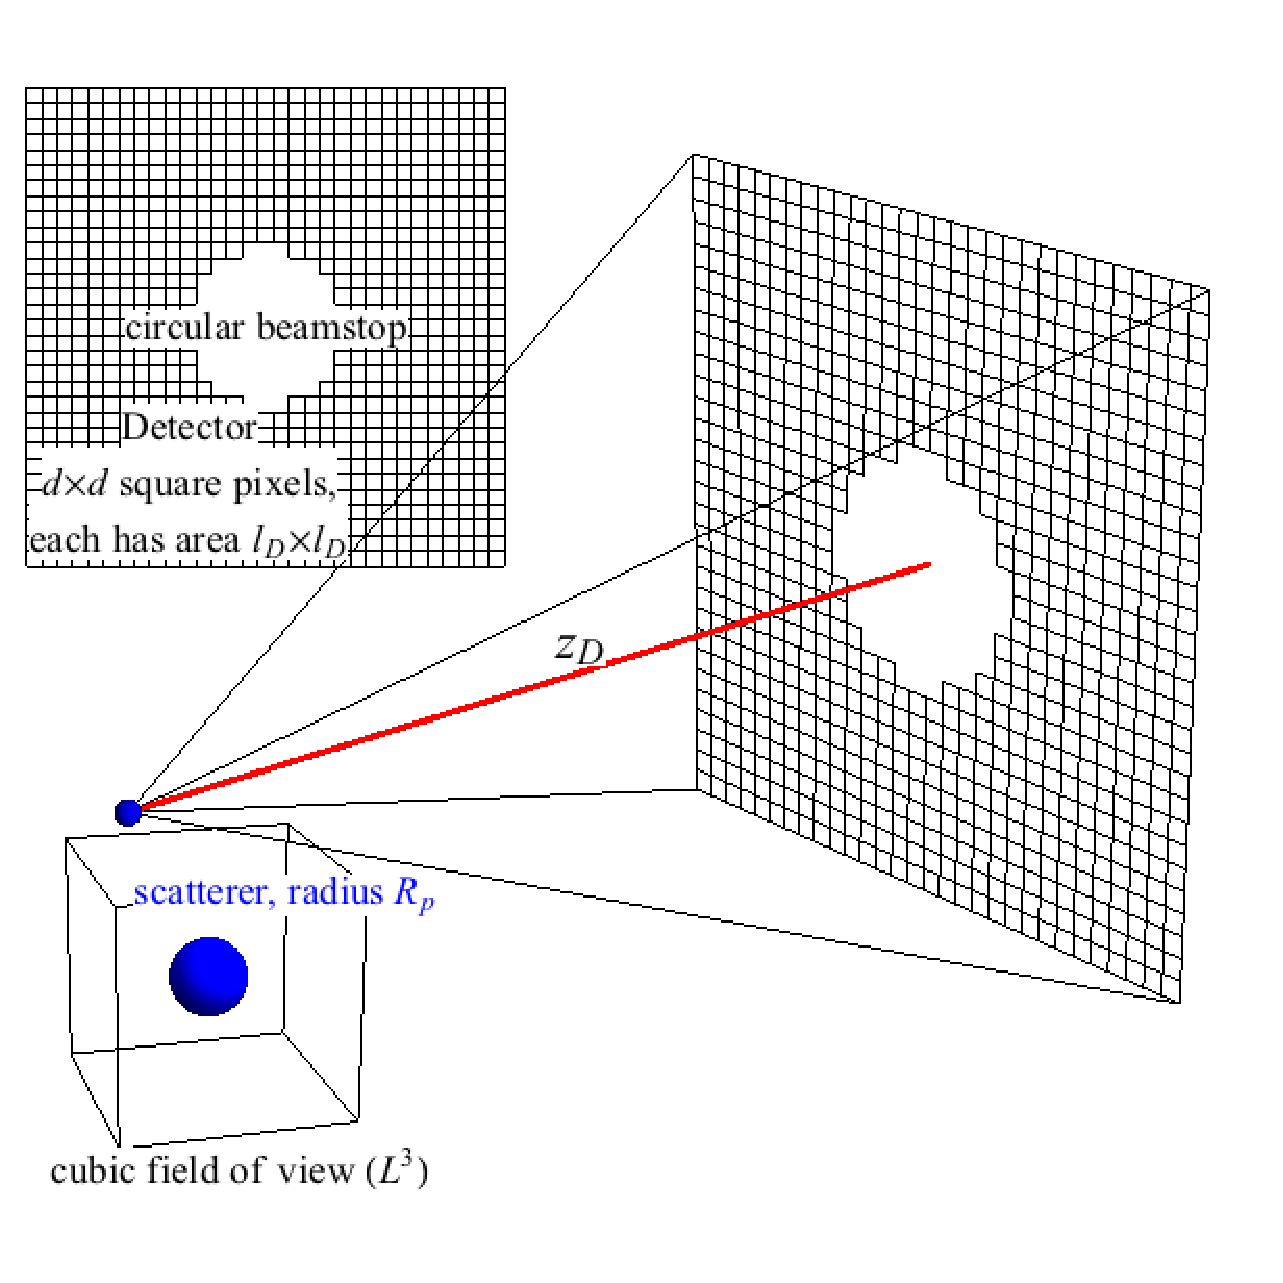
\includegraphics[width=\textwidth]{figures/geometry.eps} \label{fig:expGeometry}
\end{figure}

 %-------------------------------------------------------------------------
\begin{figure}
\caption{Flowchart to simulate a data set and perform a reconstruction starting from a sample PDB file and a configuration file, \texttt{config.ini}, with information about the experimental setup. Input and output are written in text; modules are written in boxes.}\label{fig:simFlowchart}
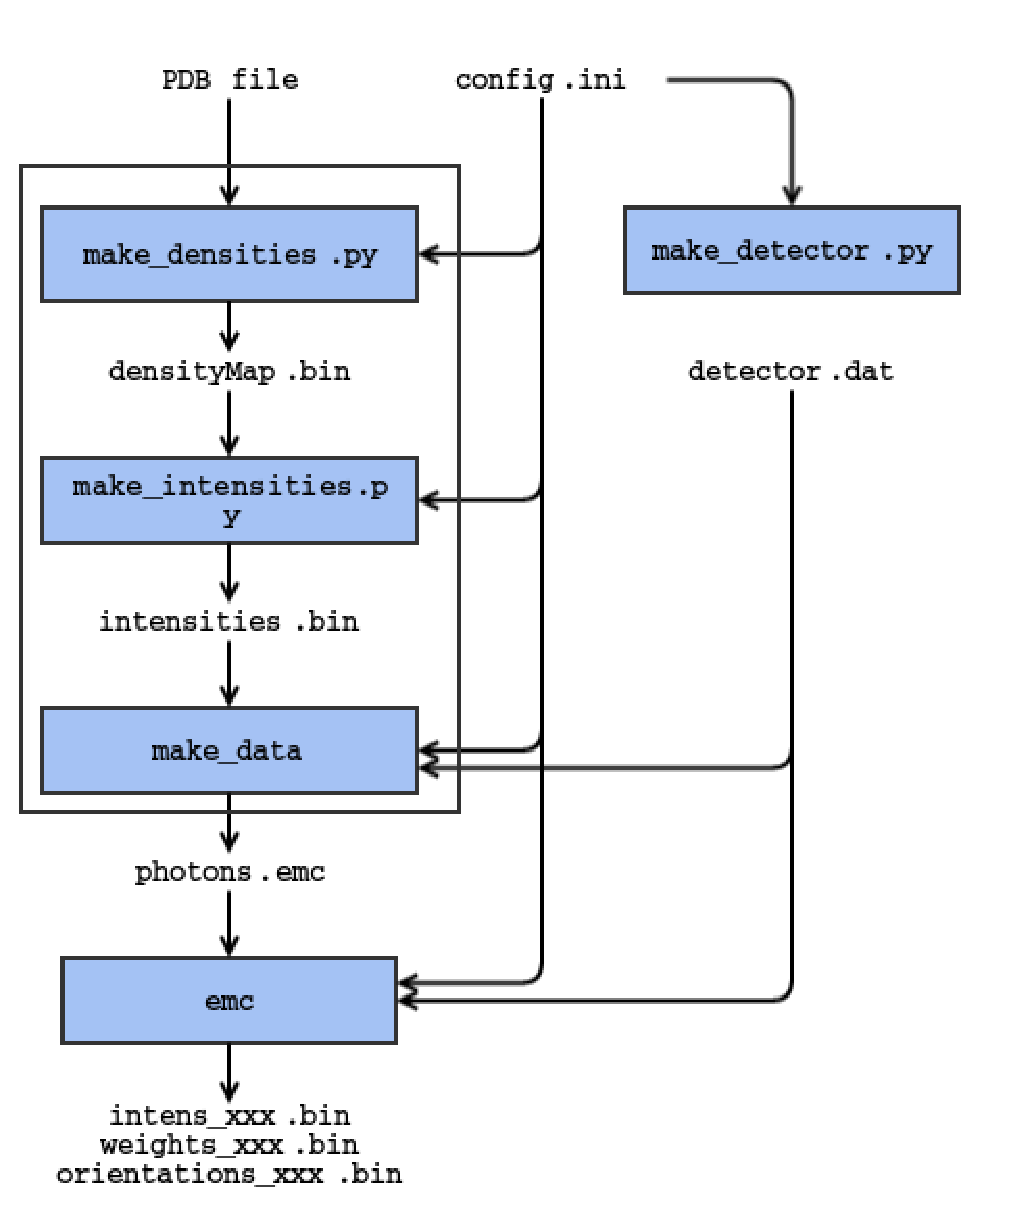
\includegraphics[width=\textwidth]{figures/emc_sim.pdf}
\end{figure}

 %-------------------------------------------------------------------------
\begin{figure}
\caption{Flowchart to process experimental data in sparse format. Information about the experimental parameters is placed in the configuration file \texttt{config.ini} and the detector geometry is in \texttt{detector.dat}. The formats of all three input files is described in Section~\ref{subsec:formats}.}\label{fig:expFlowchart}
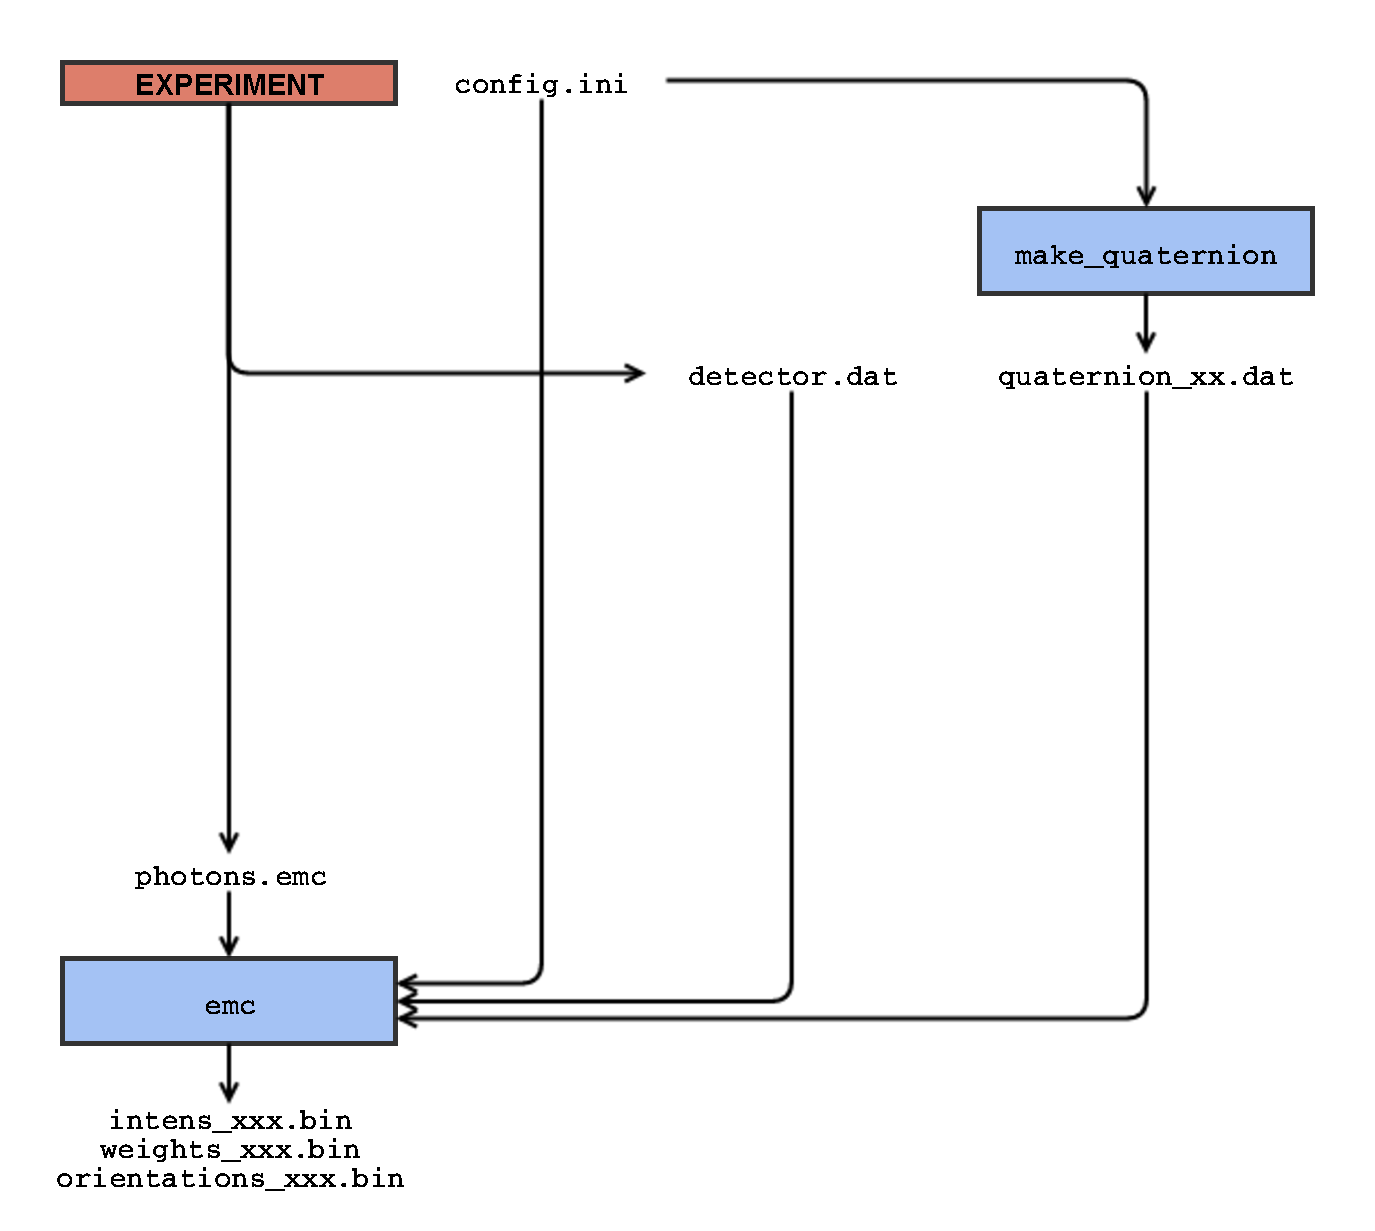
\includegraphics[width=\textwidth]{figures/emc_exp.pdf}
\end{figure}

 %-------------------------------------------------------------------------
\begin{figure}
\begin{lstlisting}[language=ini]
[parameters]
detd = 300
lambda = 6.2
detsize = 150
pixsize = 0.512
stoprad = 10
polarization = x

[make_densities]
in_pdb_file = aux/4BED.pdb
scatt_dir = aux/henke_table
out_density_file = data/densityMap.bin

[make_intensities]
in_density_file = make_densities:::out_density_file
out_intensity_file = data/intensities.bin

[make_detector]
out_detector_file = data/det_sim.dat

[make_data]
num_data = 300000
fluence = 1e10
in_detector_file = make_detector:::out_detector_file
in_intensity_file = make_intensities:::out_intensity_file
out_photons_file = data/photons.emc

[make_quaternion]
num_div = 9
out_quat_file = aux/quat_09.dat

[emc]
in_photons_file = make_data:::out_photons_file
in_detector_file = make_detector:::out_detector_file
in_quat_file = make_quaternion:::out_quat_file
out_folder = data/
log_file = EMC.log
need_scaling = 0
beta = 1.
\end{lstlisting}
\caption{Typical configuration file describing various parameters used to perform a basic simulation and reconstruction using the KLH1 (\texttt{4BED.pdb}) molecule. Compare these with numbers from Table \ref{table:simParams}.}
\label{fig:config}
\end{figure}

 %-------------------------------------------------------------------------
\begin{figure}
\caption{Six blocks in the parse data format for 50 patterns. The data is stored contiguously but shown here in row-major format (i.e. to be read from left to right, then down the rows). Each square represents a 32-bit integer. The two integers in the header block are the number of patterns, followed by number of pixels in the detector. The colors in blocks three to six connect listings of the same pattern. Details found in Section \ref{subsubsec:emcformat}.}\label{fig:dataFormat}
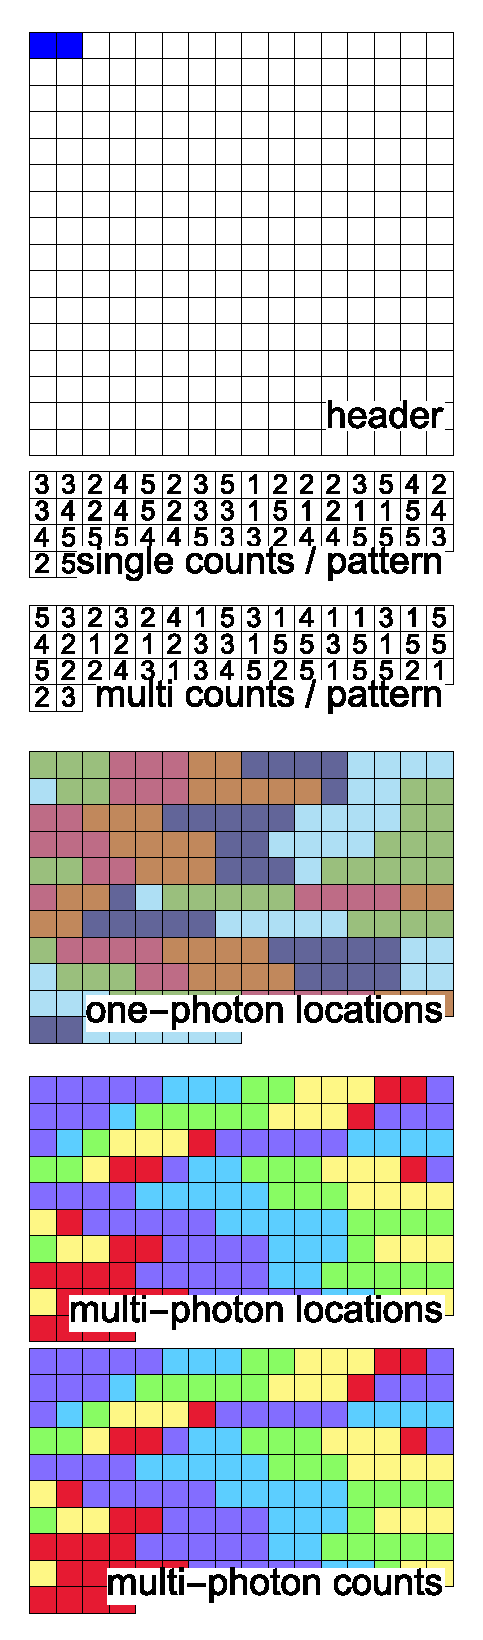
\includegraphics[height=0.8\textheight]{figures/dataFormat}
\end{figure}

 %-------------------------------------------------------------------------
\begin{table}
\caption{Parameters for EMC reconstructions of simulated single-particle imaging.} \label{table:simParams}
\label{parameters}
\begin{tabular}{p{3.5cm} p{1.4cm} p{1.4cm} p{1.4cm}}
                        			& AMO (low)          & CXI              & AMO (high)\\
\hline
photon energy (keV)     	& 2.0                 & 7.0              & 2.0 \\
$\lambda$, photon wavelength (\AA)	& 6.2                 & 1.77             & 6.2 \\
$z_D$, detector distance (mm)  	& 300                 & 350              & 290 \\
$d$, detector size (pixel)   	& 150                 & 150              & 150 \\
$l_D$, pixel side length (mm)         		& 0.512               & 0.751            & 0.512 \\
$L$, full field of view (nm) 	& 363		& 82.4		& 351 \\
beamstop radius (pixel) 	& 10.0                & 8.0              & 10.0 \\
fluence (photons/um$^2$)& $1\times10^{10}$\footnote{Estimated from \citeasnoun{Loh2013}.}    & $1\times10^{12}$ & $\mathbf{3.1\times10^{12}}$ \\
$a$, half-period resolution\footnote{Resolution defined from detector's edge.}(nm) 	& 2.45                & 0.56             & 2.5 \\
\hline
particle                  		& KLH1\footnote{Keyhole Limpet Hemocyanin 1. \label{KLH1}}& TMV\footnote{Four-layer Tobacco Mosaic Virus.}& KLH1$^\ref{KLH1}$ \\
mass (MDa)	            	& 7.3                & 1.3               & 7.3 \\
$R_p$, particle radius (nm) 		& 18.9                & 9.3                & 18.9 \\
$\widetilde{R}$\footnote{Dimensionless radius, $R_p / a$.}, dimensionless radius  & 7.7               & 16.6               & 7.6 \\
$\sigma$, speckle sampling\footnote{Defined as $\widetilde{R} = L\,/(2 R_p)$. See appendix \ref{sec:speckle}.}  & 9.6                & 4.45               & 9.2 \\
$N$, mean photons/frame & 90                  & 90               &  $\mathbf{2.8\times10^{4}}$ \\
number of data frames & $3\times 10^5$       & $5\times 10^5$    & $1\times 10^5$ \\
max. quaternion sampling\footnote{Sampling and criterion defined in \citeasnoun{loh2009}.}   & 9                   & 16                & 9 \\

\end{tabular}
\end{table}

 %-------------------------------------------------------------------------
\begin{figure}
\caption{Convergence of diffraction speckle features in a simulated AMO single-particle experiment (parameters listed in Table \ref{table:simParams}). In each row we render central slices of the 3D diffraction intensities recovered from KLH1 during an EMC reconstruction, after iterations 1,10,20 and 50 in ascending row order. The bottom plots are additional diagnostics on the reconstructed 3D diffraction model: (left column) the root mean squared change in the 3D model; (middle column) mutual information and log-likelihood of the model; (right) the most likely orientations of all the patterns.}
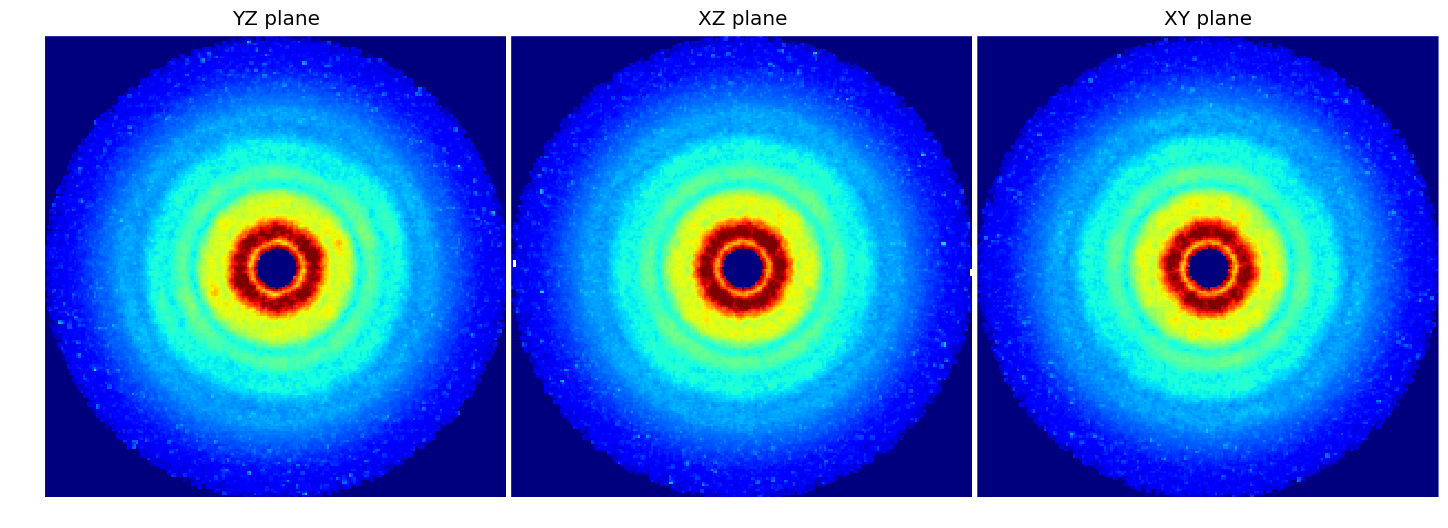
\includegraphics[height=0.13\textheight]{figures/amo_low_intens_001.png} 
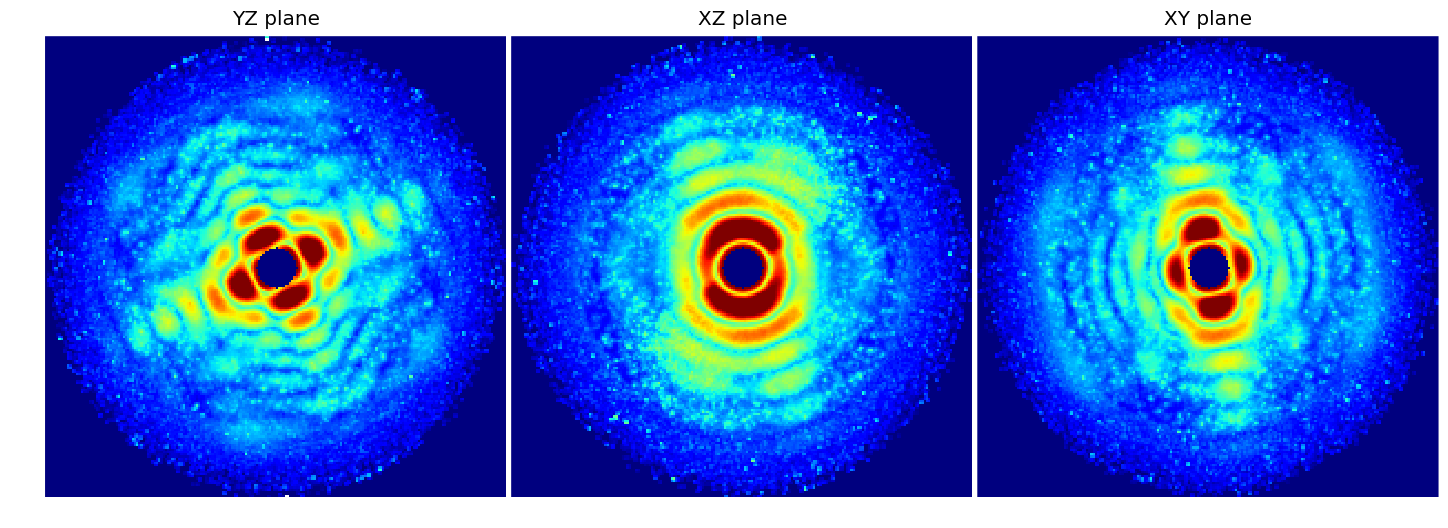
\includegraphics[height=0.13\textheight]{figures/amo_low_intens_010.png}
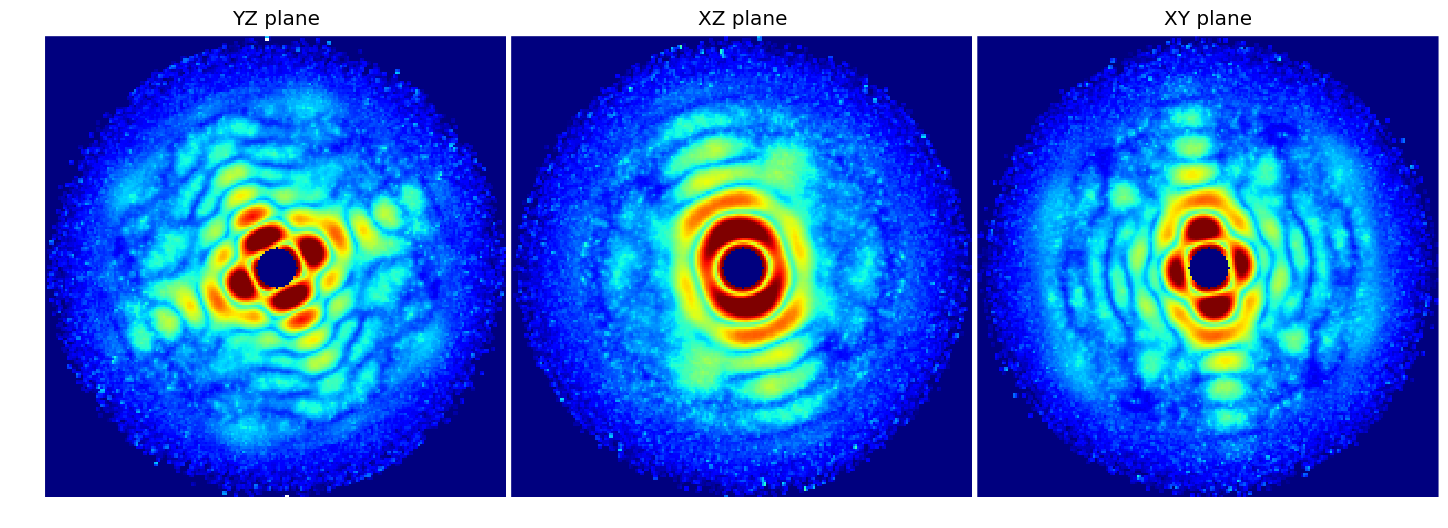
\includegraphics[height=0.13\textheight]{figures/amo_low_intens_020.png} 
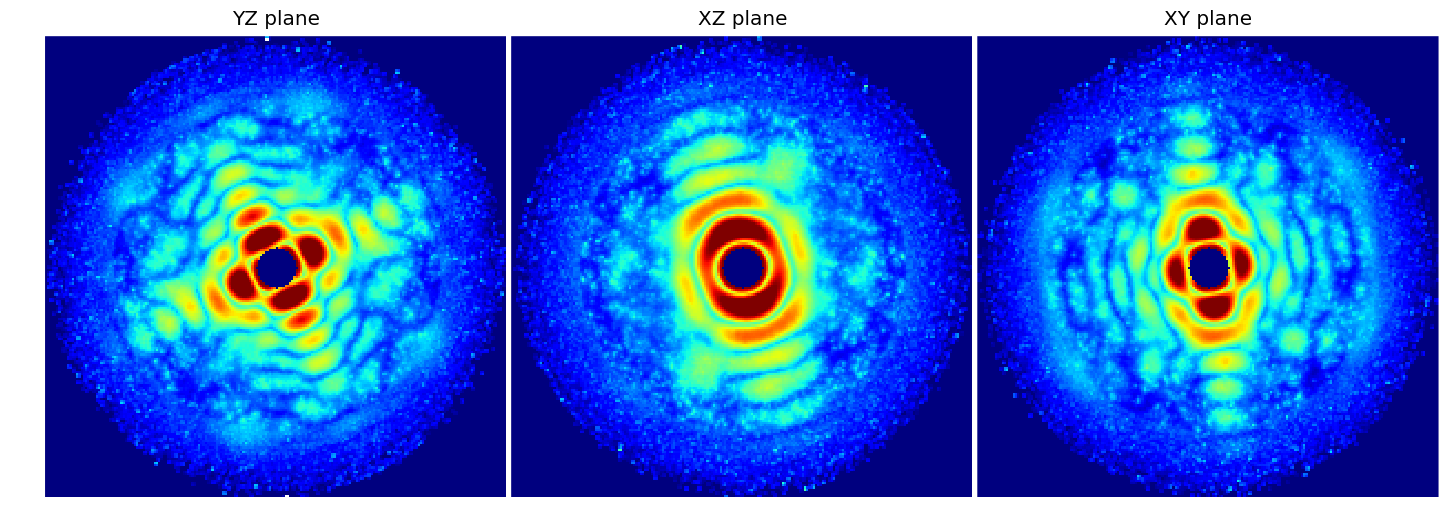
\includegraphics[height=0.13\textheight]{figures/amo_low_intens_050.png} \label{fig:amo_low_intens}
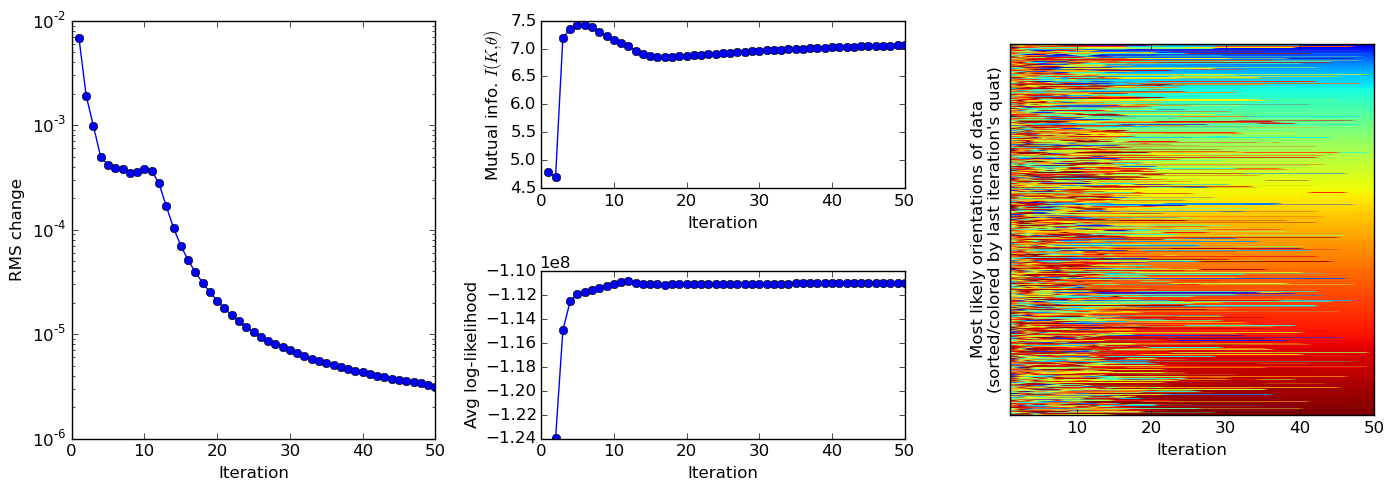
\includegraphics[height=0.13\textheight]{figures/amo_low_log.png} \label{fig:amo_low_log}
\end{figure}

 %-------------------------------------------------------------------------
\begin{figure}
\caption{The simulated reconstruction of TMV at the CXI endstation of LCLS (see Table \ref{table:simParams}). Shown here are the central sections of the reconstructed 3D diffraction volume of TMV after 55 iterations. With 88 Intel Xeon X7542 (2.67 GHz) cores this full reconstruction took 7 hours, spending 15 minutes for each of the slowest refinement iterations using 204,960 rotation group samples. Red dashed lines in the r.m.s. model change mark when the refinement level of the rotation group was increased by one. ({\bf Bottom right plot}) Rows are colored by each photon pattern's most likely orientation number, which stabilizes after twenty iterations and thereafter quickly re-stabilizes when we increase the rotation group refinement. Since the number of quaternions increase with rotation refinement, blocks of higher refinement show a wider color spectrum. See Section ~\ref{subsec:quatRefine} for details.}
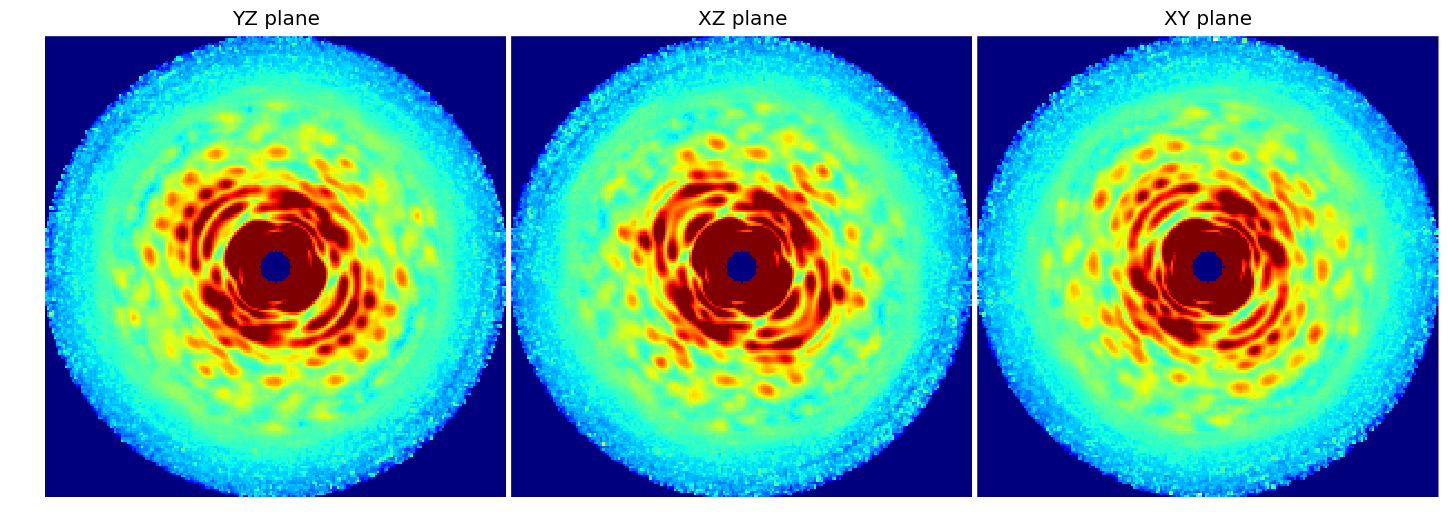
\includegraphics[width=\textwidth]{figures/cxi_intens_055.png} \label{fig:cxi_intens}
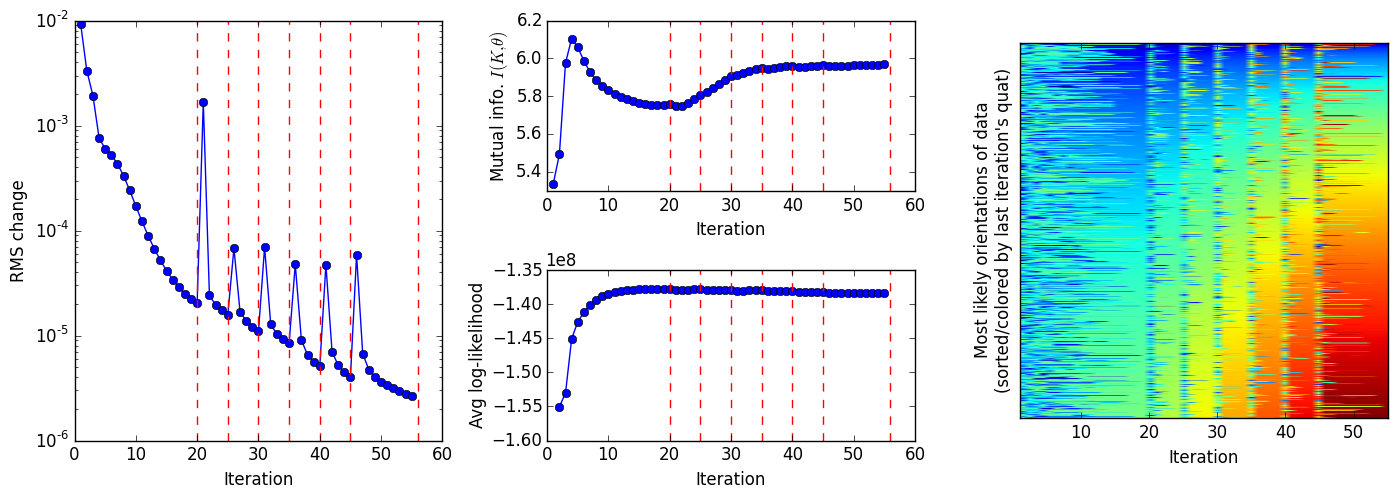
\includegraphics[width=\textwidth]{figures/cxi_log_fig.png} \label{fig:cxi_log}
\end{figure}

 %-------------------------------------------------------------------------
\begin{figure}
\caption{A simulated reconstruction at the AMO endstation at LCLS with high photon fluence (see Table \ref{table:simParams}). This reconstruction was performed by doubling the $\beta$ parameter (Section~\ref{subsec:regularization}) every 10 iterations starting from $\beta=0.001$. These iterations are indicated by dashed black lines in the log file. This interval of 10 iterations was chosen as it provided enough time for the reconstruction to stabilize before parameters were changed. This can be judged by saturation of the average mutual information in every block. After 80 iterations ($\beta = 0.256$), this increase was stopped as there did not seem to be much further improvement in the average mutual information. After this, the rotational sampling rate was increased from 6 to the target of 9. As in the CXI reconstruction (Fig.~\ref{fig:cxi_log}), this was done in order to save computational time by doing fewer iterations at the highest sampling.}
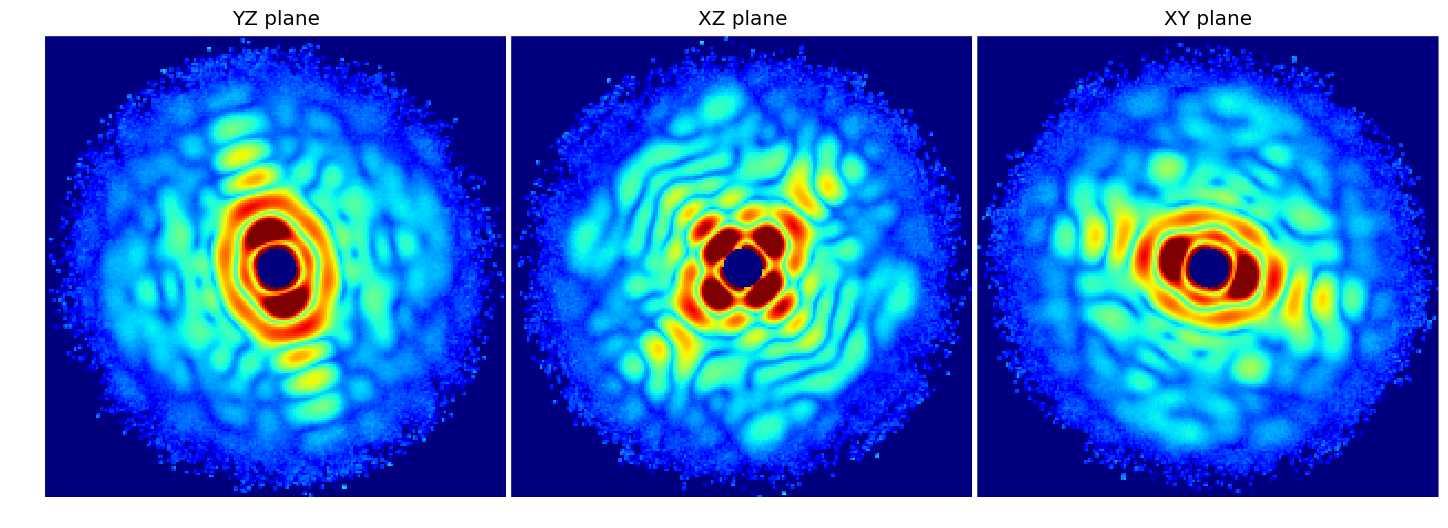
\includegraphics[width=\textwidth]{figures/amo_high_intens.png} \label{fig:amo_high_intens}
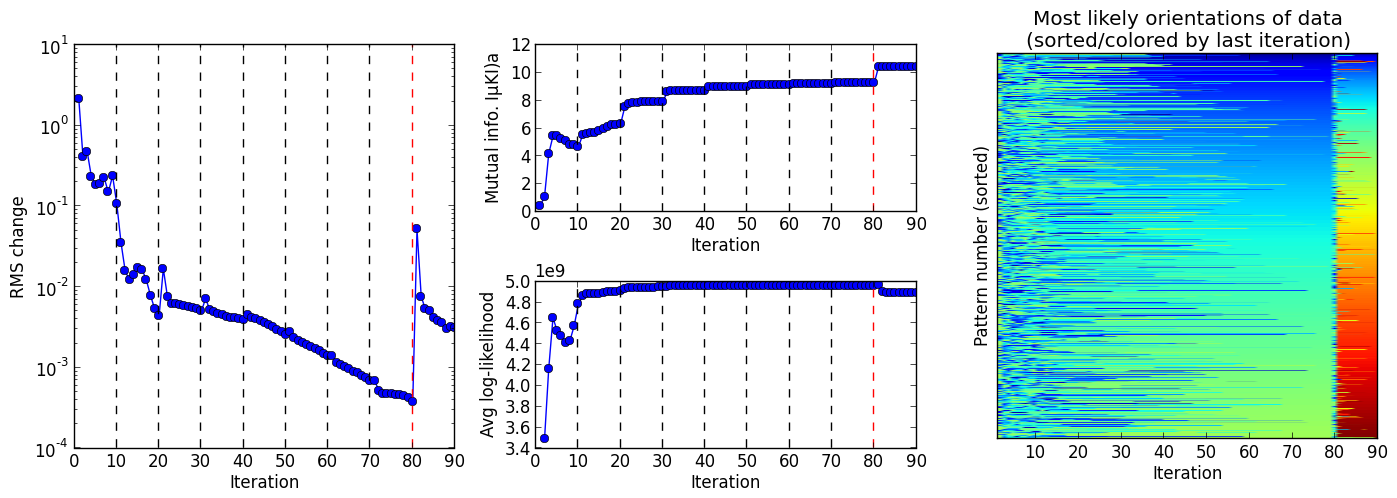
\includegraphics[width=\textwidth]{figures/amo_high_log.png} \label{fig:amo_high_log}
\end{figure}

 %-------------------------------------------------------------------------
\begin{figure}
\caption{Setup for solid angle correction. In this section we compute the solid angle subtended by the square pixel (red) on the detector plane (gray). The scatterer (blue sphere) is set at the origin of this figure.}
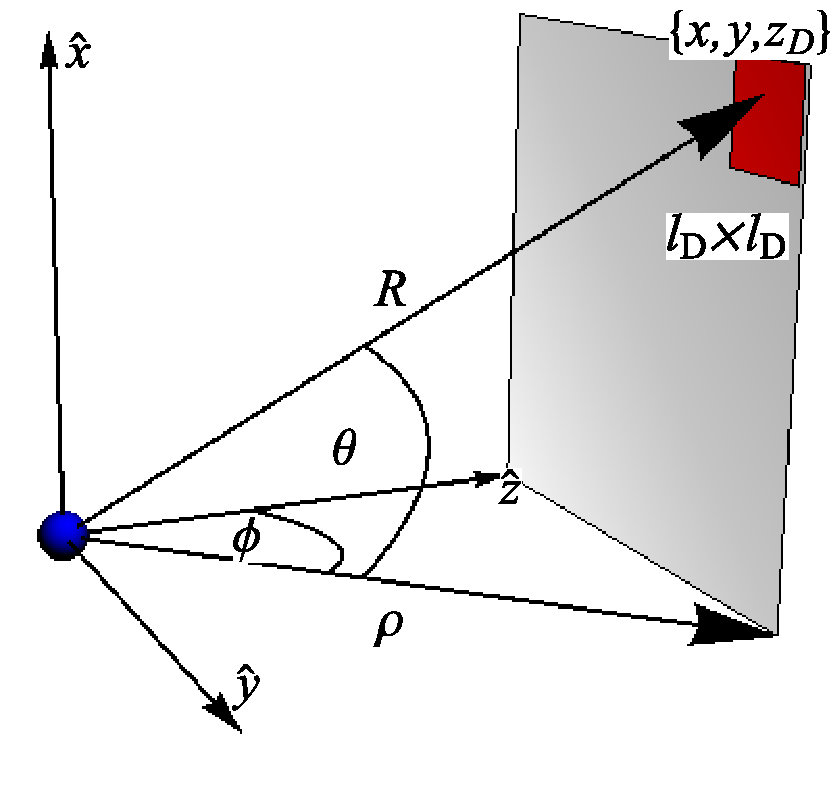
\includegraphics[width=0.8\textwidth]{figures/solidAngle.png} \label{fig:solidAngle}
\end{figure}


\end{document}                    % DO NOT DELETE THIS LINE
%%%%%%%%%%%%%%%%%%%%%%%%%%%%%%%%%%%%%%%%%%%%%%%%%%%%%%%%%%%%%%%%%%%%%%%%%%%%%%
